\documentclass{article}
\usepackage[UTF8]{ctex}
\usepackage{amsmath,mathtools,geometry,caption,tikz,float}
\geometry{a4paper,scale=0.7}

\title{每日一题(13.1)}
\author{\kaishu 李政毅}
\date{2022年4月5日}

\begin{document}
\maketitle
\textbf{1. }如图, $BD$平分$\angle ABC$, $CD$平分外角$\angle ACG$, $DE\parallel BC$交$AB$于$E$, 交$AC$于$F$.\\ (1) 线段$EF$与$BE, CF$有什么关系?\\
(2) $\angle A$与$\angle BDC$有什么关系?
\begin{figure}[H]
	\centering
	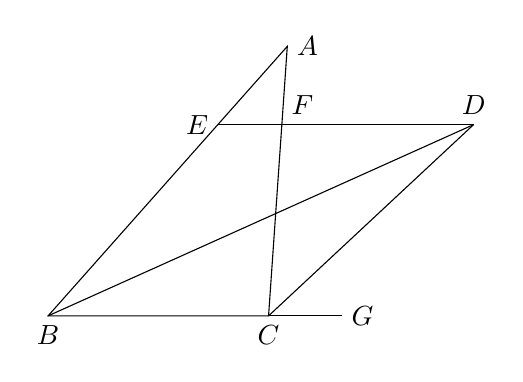
\begin{tikzpicture}[scale=0.7]
		\node at (4.34,4.89) [right] {$A$};
		\node at (0,0) [below] {$B$};
		\node at (4,0) [below] {$C$};
		\node at (7.72,3.47) [above] {$D$};
		\node at (3.08,3.47) [left] {$E$};
		\node at (4.24,3.47) [anchor=south west] {$F$};
		\node at (5.33,0) [right] {$G$};
		
		\draw (4.34,4.89)--(0,0)--(4,0)--cycle;
		\draw (4,0)--(5.33,0);
		\draw (7.72,3.47)--(3.08,3.47);
		\draw (7.72,3.47)--(0,0);
		\draw (7.72,3.47)--(4,0);
	\end{tikzpicture}
	\caption*{\kaishu 第一题图}
\end{figure}
\par
\textbf{2. }如图, $BD, CD$为外角$\angle CBM, \angle BCN$的平分线, $DE\parallel BC$交$AB$延长线于$E$, 交$AC$延长线于$F$.\\
(1) 线段$EF$与$BE, CF$有什么关系?\\
(2) $\angle A$与$\angle BDC$有什么关系?
\begin{figure}[H]
	\centering
	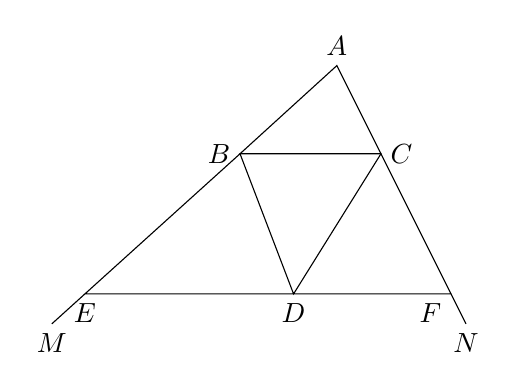
\begin{tikzpicture}[scale=1]
		\node at (3.2,2.9) [above] {$A$};
		\node at (1.97,1.78) [left] {$B$};
		\node at (3.76,1.78) [right] {$C$};
		\node at (2.65,0) [below] {$D$};
		\node at (0,0) [below] {$E$};
		\node at (4.65,0) [anchor=north east] {$F$};
		\node at (-0.42,-0.38) [below] {$M$};
		\node at (4.84,-0.38) [below] {$N$};
		
		\draw (3.2,2.9)--(1.97,1.78)--(3.76,1.78)--cycle;
		\draw (1.97,1.78)--(0,0)--(4.65,0)--(3.76,1.78)--(2.65,0)--cycle;
		\draw (0,0)--(-0.42,-0.38);
		\draw (4.65,0)--(4.84,-0.38);
	\end{tikzpicture}
	\caption*{\kaishu 第二题图}
\end{figure}

\end{document}